\section{Atividades}

\subsection{Estabelecer Tema de Investimento}

  \textbf{Descrição}: Essa atividade consiste na definição do tema de investimento a partir do Workshop de Requisitos realizado.\\
  
  \textbf{Participantes}: Product Manager, Scrum Master, Time \\
  
  \textbf{Entradas}: Modelo de negócio \\
  
  \textbf{Saídas}: Anotações do \textit{Workshop} \\

\subsection{Levantar Épicos}
  \textbf{Descrição}: Essa atividade consiste no levantamento dos épicos com o Product Manager através do Workshop de Requisitos. \\
  
  \textbf{Participantes}: Product Manager, Scrum Master, Time \\
  
  \textbf{Entradas}: Anotações do \textit{Workshop} \\
  
  \textbf{Saídas}: \textit{Backlog} do Programa \\

\subsection{Fazer reunião de validação dos épicos}
  \textbf{Descrição}: Essa atividade consiste na apresentação dos épicos especificados para o Product Manager, de modo a validar se os épicos 
  especificados estão corretos e correspondem ao esperado. \\
  
  \textbf{Participantes}: Product Manager, Scrum Master, Time \\
  
  \textbf{Entradas}: \textit{Backlog} do Programa \\
  
  \textbf{Saídas}:  Não se aplica\\

\subsection{Levantar Features}
\textbf{Descrição}: Essa atividade consiste em listar as Features, a partir dos épicos , 
que são as tarefas ou os “serviços” que o sistema deve fornecer para atender as necessidades das partes interessadas. \\

\textbf{Participantes}: Product Manager, Scrum Master, Time \\

\textbf{Entradas}: \textit{Backlog} do Programa (épicos) \\

\textbf{Saídas}:   \textit{Backlog} do Programa \\

\subsection{Especificar Features}
\textbf{Descrição}: Na especificação das features deve-se analisar e detalhar as features listadas anteriormente.
Deve-se observar se as features condizem com ou traduzem de forma clara os Épicos 
definidos previamente, e se através delas é possível escrever as Histórias de Usuário.\\

\textbf{Participantes}: Product Manager, Scrum Master, Time \\

\textbf{Entradas}: \textit{Backlog} do Programa\\

\textbf{Saídas}:   \textit{Backlog} do Programa (refinado)\\

\subsection{Fazer reunião de validação das features}
  \textbf{Descrição}: Essa atividade consiste na apresentação das features especificadas para o Product Manager, de modo a validar se 
  estão corretos e correspondem ao esperado.  \\
  
  \textbf{Participantes}: Product Manager, Scrum Master, Time \\
  
  \textbf{Entradas}: \textit{Backlog} do Programa \\
  
  \textbf{Saídas}:  Não se aplica\\
  
\subsection{Identificar Requisitos Não Funcionais}
  \textbf{Descrição}: Nesta atividade são identificados e descritos os requisitos não funcionais do sistema e são armazenados no Backlog do Programa.  \\
  
  \textbf{Participantes}: Product Manager, Scrum Master, Time \\
  
  \textbf{Entradas}:  Não se aplica\\
  
  \textbf{Saídas}:  \textit{Backlog} do Programa\\

\subsection{Construir Visão}
  \textbf{Descrição}: Nesta atividade, deve-se compilar as Features, com os requisitos não funcionais, incluindo elementos 
  regulatórios ou outros padrões de conformidade, e qualquer restrição de design. A partir disso, é possível descrever um panorama da solução a 
  ser desenvolvida, refletindo as necessidades das partes interessadas e os recursos propostos para atender essas necessidades. \\
  
  \textbf{Participantes}: Product Manager, Scrum Master, Time \\
  
  \textbf{Entradas}: \textit{Backlog} do Programa, Requisitos Não funcionais \\
  
  \textbf{Saídas}:  Visão\\
  
\subsection{Construir Roadmap}
  \textbf{Descrição}: A partir da Visão, deve-se elaborar uma espécie de roteiro, que situa e comunica a equipe e o programa em relação ao 
  alinhamento dos objetivos de negócios, e fornece visibilidade das entregas ao longo de um cronograma de curto prazo. 
  Esse roteiro divide as features nas Releases. \\
  
  \textbf{Participantes}: Product Manager, Scrum Master, Time \\
  
  \textbf{Entradas}: Visão \\
  
  \textbf{Saídas}:  Roadmap\\

\begin{figure}[!htb]
\centering
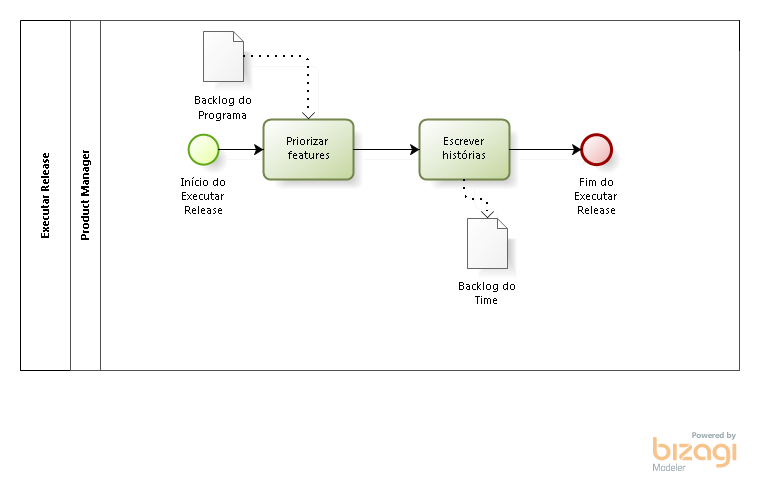
\includegraphics[scale=0.7]{figuras/release.png}
\caption{Subprocesso Executar Release}
\label{fig:release}
\end{figure}
  
A partir do Subprocesso da Figura \ref{fig:release} o processo contém as seguintes atividades.

\subsection{Priorizar features}
  \textbf{Descrição}: Essa atividade consiste na priorização das features para a Release. \\
  
  \textbf{Participantes}: Product Manager, Scrum Master\\
  
  \textbf{Entradas}: \textit{Backlog} do Programa \\
  
  \textbf{Saídas}:  Não se aplica\\

\subsection{Escrever histórias}
  \textbf{Descrição}: Essa atividade consiste na escrita das histórias em um nível macro, derivadas das features, para composição do \textit{Backlog} do Time. \\
  
  \textbf{Participantes}: Product Manager, Scrum Master\\
  
  \textbf{Entradas}: \textit{Backlog} do Programa \\
  
  \textbf{Saídas}:   \textit{Backlog} do Time \\

\begin{figure}[!htb]
\centering
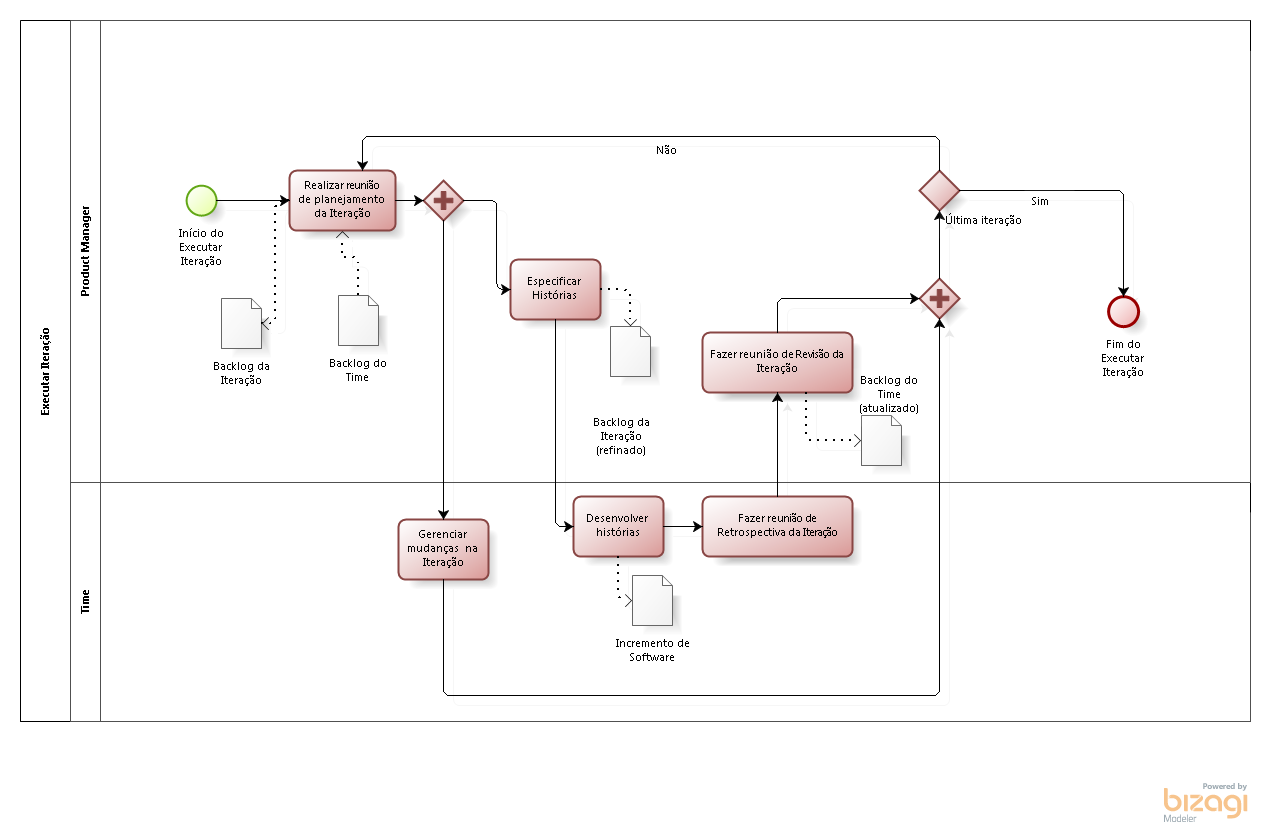
\includegraphics[scale=0.5]{figuras/iteracao.png}
\caption{Suprocesso Executar Iteração}
\label{fig:iteracao}
\end{figure}

A partir do Subprocesso da Figura \ref{fig:iteracao} o processo contém as seguintes atividades.

\subsection{Realizar reunião de planejamento da Iteração}
  \textbf{Descrição}: Essa atividade consiste no planejamento da iteração através da alocação das histórias definidas no Backlog do Time para o Backlog da Sprint. \\
  
  \textbf{Participantes}: Product Manager, Scrum Master, Time\\
  
  \textbf{Entradas}: \textit{Backlog} do Time \\
  
  \textbf{Saídas}:  \textit{Backlog} da Iteração\\

\subsection{Especificar histórias}
  \textbf{Descrição}: Essa atividade consiste na escrita mais detalhada das histórias que irão compor a 
iteração. \\
  
  \textbf{Participantes}: Product Manager, Scrum Master, Time\\
  
  \textbf{Entradas}: \textit{Backlog} da Iteração \\
  
  \textbf{Saídas}:   \textit{Backlog} da Iteração (refinado)\\

\subsection{Desenvolver histórias}
  \textbf{Descrição}: Essa atividade consiste no desenvolvimento e teste das histórias contidas no Backlog da Iteração. Tem uma duração de 1 semana. \\
  
  \textbf{Participantes}: Time\\
  
  \textbf{Entradas}: \textit{Backlog} da Iteração \\
  
  \textbf{Saídas}:   Incremento de Software\\
  
\subsection{Fazer reunião de revisão e retrospectiva da Iteração}
  \textbf{Descrição}: Essa atividade consiste na validação das histórias implementadas através da execução dos testes de aceitação. \\
  
  \textbf{Participantes}: Product Manager, Time\\
  
  \textbf{Entradas}: Incremento de Software \\
  
  \textbf{Saídas}:   \textit{Backlog} da Iteração (atualizado)\\
